% Please provide your report for the architecture assignment here.  Please make sure you:

% Describe the you are assigned.  Don't go to small details.  Cover only basic components
% Describe how the data is passed
% Describe the messaging between the components.
% For the bug assigned to you, describe what it is, how to reproduce and a possible solution.
% I expect your report to be 2-4 pages.

\documentclass[a4paper, 11pt]{article}
%% Math Support
\usepackage{amssymb}
\usepackage{amsmath}
\usepackage{enumitem}
%% antifloat image
\usepackage{float}
%[H] for fix 
%[htbp] for float

%% Graphics Support
\usepackage{listings}%begin MATLAB 
\usepackage{color}
\usepackage{placeins}

\definecolor{dkgreen}{rgb}{0,0.6,0}
\definecolor{gray}{rgb}{0.5,0.5,0.5}
\definecolor{mauve}{rgb}{0.58,0,0.82}

\lstset{frame=tb,
language=MATLAB,
aboveskip=3mm,
belowskip=3mm,
showstringspaces=false,
columns=flexible,
basicstyle={\small\ttfamily},
numbers=none,
numberstyle=\tiny\color{gray},
keywordstyle=\color{blue},
commentstyle=\color{dkgreen},
stringstyle=\color{mauve},
breaklines=true,
breakatwhitespace=true,
tabsize=3
}%end MATLAB 
\setlength\parindent{0pt}
\usepackage{color}
\usepackage{xcolor}
\usepackage{graphicx}  % png/jpg support
\usepackage{fullpage} % changes the margin
\setcounter{section}{0}

\begin{document}

\large\textbf{EC 500 C1 Building Software}
\hfill
\today
\hfill
\textbf{Bowen Song U04079758}

{\section*{}}
\begin{title}
	\centering
    \vspace*{0.5cm}

    \huge\bfseries
    \centering Archtecture Assignment: MoviePy\footnote{This review is done under docker MoviePy environment.}

    \vspace*{0.5cm}
\end{title}
\noindent

\section{Overview}

The MoviePy is a Python API library that helps to edit movies. The input could be images or videos and output could be videos of different formats. This API is built based on the following several dependencies:
\begin{itemize}
	\item \textit{numpy} - calculations and manipulations
	\item \textit{imageio} - reading and writing images of different format
	\item \textit{Decorator} - sync manipulation over videos on masks
	\item \textit{tqdm} - showing video progress progress on command-line UI
	\item \textit{youtube\_dl} - interacting with Youtube
	\item \textit{Sphinx} - creating \textit{MoviePy} documentation
	\item \textit{requests} - opening URL
	\item \textit{ffmpeg} - processing video. 
\end{itemize}

The Main components and their building blocks including:
\begin{itemize}
   \item VideoClip - Image, Color, and Text
   \item AudioClip - Audio File and Composite Audio
   \item videofx - Video effects
   \item audiofx - Fade effect, looping, and volume
   \item videotools - Credits, drawing, segmenting, subtitles, and tracking
   \item audiotools - Not implemented
   \item ffmpeg - ffmpeg Tools for audio extraction, sub-clip extraction, merger video and audio, form video by frame, and resizing a video
   \item decorators - apply functions to mask and video
\end{itemize}
\section{Architecture}
The movie editing test came out with interaction with API components as shown in Figure \ref{figure:graph}.

\begin{figure}[ht]
  \centering
  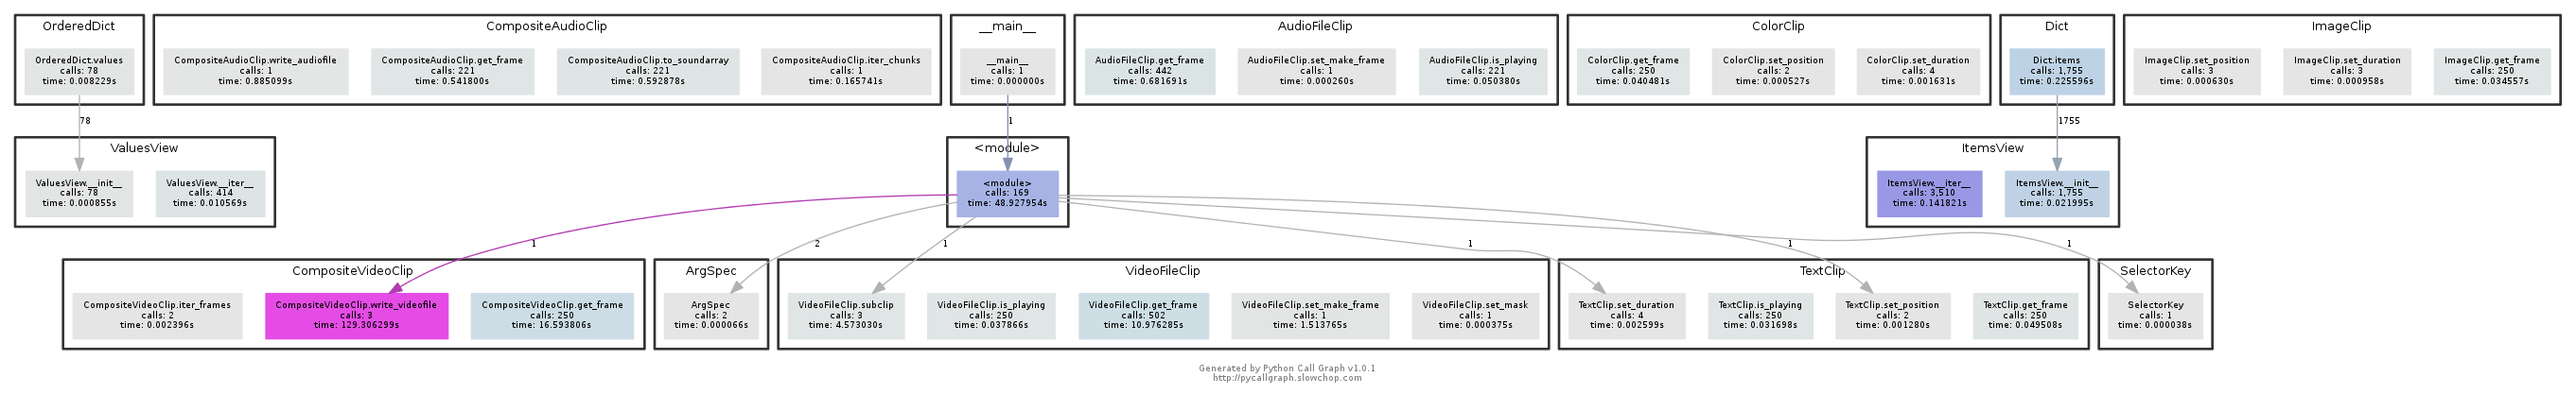
\includegraphics[width=\linewidth]{pycallgraph.png}
  \caption{Architecture}
   \label{figure:graph}
  \end{figure}
\FloatBarrier

This architecture flow graph outlines the function calls going through each involved component of the API. The test file resized a video input and output into a video in a different format. The main function source code is presented as the following.

\begin{lstlisting}
#!/usr/bin/env python3
from moviepy.editor import *

video = VideoFileClip("myHolidays.mkv").subclip(50,60)

# Make the text. Many more options are available.
txt_clip = ( TextClip("My Holidays 2013",fontsize=70,color='white')
             .set_position('center')
             .set_duration(10) )

result = CompositeVideoClip([video, txt_clip]) # Overlay text on video
result.write_videofile("myHolidays_edited.webm",fps=25) # Many options...
\end{lstlisting}

The flow graph starts from the middle where the \textit{\_\_main\_\_} module calls for components (Class): Composite Video Clip, Video Clip, and Text Clip. Within each class, several functions can be invoked. This specific main function invokes one to two functions in each class. However, inside the class, each function may be called by each other for several times and is shown on the flow graph. The ones not directly called but triggered by other functions in this specific main function are listed at the top.


\section{Issue \#640}
The issue \#640 is created regarding clip resizing function in file the ``resize.py''. This function plays an important role in video processing procedure. The issue for the function is considered bug and was proposed a fix for it. It is more of a pull request than an issue since a solution is proposed. \\

The problem code piece is attached as follow:

\begin{lstlisting}
newsize2 = lambda t : trans_newsize(newsize(t))

        if clip.ismask:

            fun = lambda gf,t: (1.0*resizer((255 * gf(t)).astype('uint8'),
                                             newsize2(t))/255)

        else:

            fun = lambda gf,t: resizer(gf(t).astype('uint8'),
                                      newsize2(t))

        return clip.fl(fun, keep_duration=True,
                       apply_to= (["mask"] if apply_to_mask else []))
\end{lstlisting}.

The issuer claims that the function fails for mask frames in the \textit{else} argument. However, the \textit{else} statement should not process any clip with a mask as the leading \textit{if} statement is directing all the clip with mask into the first statement. The \textit{else} statement should not handle any clips with a mask. \\

Nevertheless, the proposed solution is attached as below. The issuer copied handle from \textit{ismask} statement to the else in an attempt to band-aid the error.
\begin{lstlisting}
 newsize2 = lambda t : trans_newsize(newsize(t))
        if clip.ismask:
            
            fun = lambda gf,t: (1.0*resizer((255 * gf(t)).astype('uint8'),
                                             newsize2(t))/255)

        else:
            
            fun = lambda gf,t: resizer(gf(t).astype('uint8'),
                                  newsize2(t)) if len(gf(t).shape) == 3 else 1.0*resizer((gf(t)*255).astype('uint8'),newsize2(t))/255

        return clip.fl(fun, keep_duration=True,
                       apply_to= (["mask"] if apply_to_mask else []))`
\end{lstlisting}


\end{document}  